
%% bare_jrnl.tex
%% V1.3
%% 2007/01/11
%% by Michael Shell
%% see http://www.michaelshell.org/
%% for current contact information.
%%
%% This is a skeleton file demonstrating the use of IEEEtran.cls
%% (requires IEEEtran.cls version 1.7 or later) with an IEEE journal paper.
%%
%% Support sites:
%% http://www.michaelshell.org/tex/ieeetran/
%% http://www.ctan.org/tex-archive/macros/latex/contrib/IEEEtran/
%% and
%% http://www.ieee.org/



% *** Authors should verify (and, if needed, correct) their LaTeX system  ***
% *** with the testflow diagnostic prior to trusting their LaTeX platform ***
% *** with production work. IEEE's font choices can trigger bugs that do  ***
% *** not appear when using other class files.                            ***
% The testflow support page is at:
% http://www.michaelshell.org/tex/testflow/


%%*************************************************************************
%% Legal Notice:
%% This code is offered as-is without any warranty either expressed or
%% implied; without even the implied warranty of MERCHANTABILITY or
%% FITNESS FOR A PARTICULAR PURPOSE! 
%% User assumes all risk.
%% In no event shall IEEE or any contributor to this code be liable for
%% any damages or losses, including, but not limited to, incidental,
%% consequential, or any other damages, resulting from the use or misuse
%% of any information contained here.
%%
%% All comments are the opinions of their respective authors and are not
%% necessarily endorsed by the IEEE.
%%
%% This work is distributed under the LaTeX Project Public License (LPPL)
%% ( http://www.latex-project.org/ ) version 1.3, and may be freely used,
%% distributed and modified. A copy of the LPPL, version 1.3, is included
%% in the base LaTeX documentation of all distributions of LaTeX released
%% 2003/12/01 or later.
%% Retain all contribution notices and credits.
%% ** Modified files should be clearly indicated as such, including  **
%% ** renaming them and changing author support contact information. **
%%
%% File list of work: IEEEtran.cls, IEEEtran_HOWTO.pdf, bare_adv.tex,
%%                    bare_conf.tex, bare_jrnl.tex, bare_jrnl_compsoc.tex
%%*************************************************************************

% Note that the a4paper option is mainly intended so that authors in
% countries using A4 can easily print to A4 and see how their papers will
% look in print - the typesetting of the document will not typically be
% affected with changes in paper size (but the bottom and side margins will).
% Use the testflow package mentioned above to verify correct handling of
% both paper sizes by the user's LaTeX system.
%
% Also note that the "draftcls" or "draftclsnofoot", not "draft", option
% should be used if it is desired that the figures are to be displayed in
% draft mode.
%
\documentclass[journal]{IEEEtran}
\usepackage{blindtext}
\usepackage{graphicx}

% Some very useful LaTeX packages include:
% (uncomment the ones you want to load)


% *** MISC UTILITY PACKAGES ***
%
%\usepackage{ifpdf}
% Heiko Oberdiek's ifpdf.sty is very useful if you need conditional
% compilation based on whether the output is pdf or dvi.
% usage:
% \ifpdf
%   % pdf code
% \else
%   % dvi code
% \fi
% The latest version of ifpdf.sty can be obtained from:
% http://www.ctan.org/tex-archive/macros/latex/contrib/oberdiek/
% Also, note that IEEEtran.cls V1.7 and later provides a builtin
% \ifCLASSINFOpdf conditional that works the same way.
% When switching from latex to pdflatex and vice-versa, the compiler may
% have to be run twice to clear warning/error messages.






% *** CITATION PACKAGES ***
%
%\usepackage{cite}
% cite.sty was written by Donald Arseneau
% V1.6 and later of IEEEtran pre-defines the format of the cite.sty package
% \cite{} output to follow that of IEEE. Loading the cite package will
% result in citation numbers being automatically sorted and properly
% "compressed/ranged". e.g., [1], [9], [2], [7], [5], [6] without using
% cite.sty will become [1], [2], [5]--[7], [9] using cite.sty. cite.sty's
% \cite will automatically add leading space, if needed. Use cite.sty's
% noadjust option (cite.sty V3.8 and later) if you want to turn this off.
% cite.sty is already installed on most LaTeX systems. Be sure and use
% version 4.0 (2003-05-27) and later if using hyperref.sty. cite.sty does
% not currently provide for hyperlinked citations.
% The latest version can be obtained at:
% http://www.ctan.org/tex-archive/macros/latex/contrib/cite/
% The documentation is contained in the cite.sty file itself.






% *** GRAPHICS RELATED PACKAGES ***
%
\ifCLASSINFOpdf
  % \usepackage[pdftex]{graphicx}
  % declare the path(s) where your graphic files are
  % \graphicspath{{../pdf/}{../jpeg/}}
  % and their extensions so you won't have to specify these with
  % every instance of \includegraphics
  % \DeclareGraphicsExtensions{.pdf,.jpeg,.png}
\else
  % or other class option (dvipsone, dvipdf, if not using dvips). graphicx
  % will default to the driver specified in the system graphics.cfg if no
  % driver is specified.
  % \usepackage[dvips]{graphicx}
  % declare the path(s) where your graphic files are
  % \graphicspath{{../eps/}}
  % and their extensions so you won't have to specify these with
  % every instance of \includegraphics
  % \DeclareGraphicsExtensions{.eps}
\fi
% graphicx was written by David Carlisle and Sebastian Rahtz. It is
% required if you want graphics, photos, etc. graphicx.sty is already
% installed on most LaTeX systems. The latest version and documentation can
% be obtained at: 
% http://www.ctan.org/tex-archive/macros/latex/required/graphics/
% Another good source of documentation is "Using Imported Graphics in
% LaTeX2e" by Keith Reckdahl which can be found as epslatex.ps or
% epslatex.pdf at: http://www.ctan.org/tex-archive/info/
%
% latex, and pdflatex in dvi mode, support graphics in encapsulated
% postscript (.eps) format. pdflatex in pdf mode supports graphics
% in .pdf, .jpeg, .png and .mps (metapost) formats. Users should ensure
% that all non-photo figures use a vector format (.eps, .pdf, .mps) and
% not a bitmapped formats (.jpeg, .png). IEEE frowns on bitmapped formats
% which can result in "jaggedy"/blurry rendering of lines and letters as
% well as large increases in file sizes.
%
% You can find documentation about the pdfTeX application at:
% http://www.tug.org/applications/pdftex





% *** MATH PACKAGES ***
%
%\usepackage[cmex10]{amsmath}
% A popular package from the American Mathematical Society that provides
% many useful and powerful commands for dealing with mathematics. If using
% it, be sure to load this package with the cmex10 option to ensure that
% only type 1 fonts will utilized at all point sizes. Without this option,
% it is possible that some math symbols, particularly those within
% footnotes, will be rendered in bitmap form which will result in a
% document that can not be IEEE Xplore compliant!
%
% Also, note that the amsmath package sets \interdisplaylinepenalty to 10000
% thus preventing page breaks from occurring within multiline equations. Use:
%\interdisplaylinepenalty=2500
% after loading amsmath to restore such page breaks as IEEEtran.cls normally
% does. amsmath.sty is already installed on most LaTeX systems. The latest
% version and documentation can be obtained at:
% http://www.ctan.org/tex-archive/macros/latex/required/amslatex/math/





% *** SPECIALIZED LIST PACKAGES ***
%
%\usepackage{algorithmic}
% algorithmic.sty was written by Peter Williams and Rogerio Brito.
% This package provides an algorithmic environment fo describing algorithms.
% You can use the algorithmic environment in-text or within a figure
% environment to provide for a floating algorithm. Do NOT use the algorithm
% floating environment provided by algorithm.sty (by the same authors) or
% algorithm2e.sty (by Christophe Fiorio) as IEEE does not use dedicated
% algorithm float types and packages that provide these will not provide
% correct IEEE style captions. The latest version and documentation of
% algorithmic.sty can be obtained at:
% http://www.ctan.org/tex-archive/macros/latex/contrib/algorithms/
% There is also a support site at:
% http://algorithms.berlios.de/index.html
% Also of interest may be the (relatively newer and more customizable)
% algorithmicx.sty package by Szasz Janos:
% http://www.ctan.org/tex-archive/macros/latex/contrib/algorithmicx/




% *** ALIGNMENT PACKAGES ***
%
%\usepackage{array}
% Frank Mittelbach's and David Carlisle's array.sty patches and improves
% the standard LaTeX2e array and tabular environments to provide better
% appearance and additional user controls. As the default LaTeX2e table
% generation code is lacking to the point of almost being broken with
% respect to the quality of the end results, all users are strongly
% advised to use an enhanced (at the very least that provided by array.sty)
% set of table tools. array.sty is already installed on most systems. The
% latest version and documentation can be obtained at:
% http://www.ctan.org/tex-archive/macros/latex/required/tools/


%\usepackage{mdwmath}
%\usepackage{mdwtab}
% Also highly recommended is Mark Wooding's extremely powerful MDW tools,
% especially mdwmath.sty and mdwtab.sty which are used to format equations
% and tables, respectively. The MDWtools set is already installed on most
% LaTeX systems. The lastest version and documentation is available at:
% http://www.ctan.org/tex-archive/macros/latex/contrib/mdwtools/


% IEEEtran contains the IEEEeqnarray family of commands that can be used to
% generate multiline equations as well as matrices, tables, etc., of high
% quality.


%\usepackage{eqparbox}
% Also of notable interest is Scott Pakin's eqparbox package for creating
% (automatically sized) equal width boxes - aka "natural width parboxes".
% Available at:
% http://www.ctan.org/tex-archive/macros/latex/contrib/eqparbox/





% *** SUBFIGURE PACKAGES ***
%\usepackage[tight,footnotesize]{subfigure}
% subfigure.sty was written by Steven Douglas Cochran. This package makes it
% easy to put subfigures in your figures. e.g., "Figure 1a and 1b". For IEEE
% work, it is a good idea to load it with the tight package option to reduce
% the amount of white space around the subfigures. subfigure.sty is already
% installed on most LaTeX systems. The latest version and documentation can
% be obtained at:
% http://www.ctan.org/tex-archive/obsolete/macros/latex/contrib/subfigure/
% subfigure.sty has been superceeded by subfig.sty.



%\usepackage[caption=false]{caption}
%\usepackage[font=footnotesize]{subfig}
% subfig.sty, also written by Steven Douglas Cochran, is the modern
% replacement for subfigure.sty. However, subfig.sty requires and
% automatically loads Axel Sommerfeldt's caption.sty which will override
% IEEEtran.cls handling of captions and this will result in nonIEEE style
% figure/table captions. To prevent this problem, be sure and preload
% caption.sty with its "caption=false" package option. This is will preserve
% IEEEtran.cls handing of captions. Version 1.3 (2005/06/28) and later 
% (recommended due to many improvements over 1.2) of subfig.sty supports
% the caption=false option directly:
%\usepackage[caption=false,font=footnotesize]{subfig}
%
% The latest version and documentation can be obtained at:
% http://www.ctan.org/tex-archive/macros/latex/contrib/subfig/
% The latest version and documentation of caption.sty can be obtained at:
% http://www.ctan.org/tex-archive/macros/latex/contrib/caption/




% *** FLOAT PACKAGES ***
%
%\usepackage{fixltx2e}
% fixltx2e, the successor to the earlier fix2col.sty, was written by
% Frank Mittelbach and David Carlisle. This package corrects a few problems
% in the LaTeX2e kernel, the most notable of which is that in current
% LaTeX2e releases, the ordering of single and double column floats is not
% guaranteed to be preserved. Thus, an unpatched LaTeX2e can allow a
% single column figure to be placed prior to an earlier double column
% figure. The latest version and documentation can be found at:
% http://www.ctan.org/tex-archive/macros/latex/base/



%\usepackage{stfloats}
% stfloats.sty was written by Sigitas Tolusis. This package gives LaTeX2e
% the ability to do double column floats at the bottom of the page as well
% as the top. (e.g., "\begin{figure*}[!b]" is not normally possible in
% LaTeX2e). It also provides a command:
%\fnbelowfloat
% to enable the placement of footnotes below bottom floats (the standard
% LaTeX2e kernel puts them above bottom floats). This is an invasive package
% which rewrites many portions of the LaTeX2e float routines. It may not work
% with other packages that modify the LaTeX2e float routines. The latest
% version and documentation can be obtained at:
% http://www.ctan.org/tex-archive/macros/latex/contrib/sttools/
% Documentation is contained in the stfloats.sty comments as well as in the
% presfull.pdf file. Do not use the stfloats baselinefloat ability as IEEE
% does not allow \baselineskip to stretch. Authors submitting work to the
% IEEE should note that IEEE rarely uses double column equations and
% that authors should try to avoid such use. Do not be tempted to use the
% cuted.sty or midfloat.sty packages (also by Sigitas Tolusis) as IEEE does
% not format its papers in such ways.


%\ifCLASSOPTIONcaptionsoff
%  \usepackage[nomarkers]{endfloat}
% \let\MYoriglatexcaption\caption
% \renewcommand{\caption}[2][\relax]{\MYoriglatexcaption[#2]{#2}}
%\fi
% endfloat.sty was written by James Darrell McCauley and Jeff Goldberg.
% This package may be useful when used in conjunction with IEEEtran.cls'
% captionsoff option. Some IEEE journals/societies require that submissions
% have lists of figures/tables at the end of the paper and that
% figures/tables without any captions are placed on a page by themselves at
% the end of the document. If needed, the draftcls IEEEtran class option or
% \CLASSINPUTbaselinestretch interface can be used to increase the line
% spacing as well. Be sure and use the nomarkers option of endfloat to
% prevent endfloat from "marking" where the figures would have been placed
% in the text. The two hack lines of code above are a slight modification of
% that suggested by in the endfloat docs (section 8.3.1) to ensure that
% the full captions always appear in the list of figures/tables - even if
% the user used the short optional argument of \caption[]{}.
% IEEE papers do not typically make use of \caption[]'s optional argument,
% so this should not be an issue. A similar trick can be used to disable
% captions of packages such as subfig.sty that lack options to turn off
% the subcaptions:
% For subfig.sty:
% \let\MYorigsubfloat\subfloat
% \renewcommand{\subfloat}[2][\relax]{\MYorigsubfloat[]{#2}}
% For subfigure.sty:
% \let\MYorigsubfigure\subfigure
% \renewcommand{\subfigure}[2][\relax]{\MYorigsubfigure[]{#2}}
% However, the above trick will not work if both optional arguments of
% the \subfloat/subfig command are used. Furthermore, there needs to be a
% description of each subfigure *somewhere* and endfloat does not add
% subfigure captions to its list of figures. Thus, the best approach is to
% avoid the use of subfigure captions (many IEEE journals avoid them anyway)
% and instead reference/explain all the subfigures within the main caption.
% The latest version of endfloat.sty and its documentation can obtained at:
% http://www.ctan.org/tex-archive/macros/latex/contrib/endfloat/
%
% The IEEEtran \ifCLASSOPTIONcaptionsoff conditional can also be used
% later in the document, say, to conditionally put the References on a 
% page by themselves.





% *** PDF, URL AND HYPERLINK PACKAGES ***
%
%\usepackage{url}
% url.sty was written by Donald Arseneau. It provides better support for
% handling and breaking URLs. url.sty is already installed on most LaTeX
% systems. The latest version can be obtained at:
% http://www.ctan.org/tex-archive/macros/latex/contrib/misc/
% Read the url.sty source comments for usage information. Basically,
% \url{my_url_here}.





% *** Do not adjust lengths that control margins, column widths, etc. ***
% *** Do not use packages that alter fonts (such as pslatex).         ***
% There should be no need to do such things with IEEEtran.cls V1.6 and later.
% (Unless specifically asked to do so by the journal or conference you plan
% to submit to, of course. )


% correct bad hyphenation here
\hyphenation{op-tical net-works semi-conduc-tor}


\newcommand\norm[1]{\left\lVert#1\right\rVert}

\begin{document}
%
% paper title
% can use linebreaks \\ within to get better formatting as desired
\title{Optimization and Data Analytics\\A research project on image classification}
%
%
% author names and IEEE memberships
% note positions of commas and nonbreaking spaces ( ~ ) LaTeX will not break
% a structure at a ~ so this keeps an author's name from being broken across
% two lines.
% use \thanks{} to gain access to the first footnote area
% a separate \thanks must be used for each paragraph as LaTeX2e's \thanks
% was not built to handle multiple paragraphs
%

\author{Theo Morales [201703024]}

% note the % following the last \IEEEmembership and also \thanks - 
% these prevent an unwanted space from occurring between the last author name
% and the end of the author line. i.e., if you had this:
% 
% \author{....lastname \thanks{...} \thanks{...} }
%                     ^------------^------------^----Do not want these spaces!
%
% a space would be appended to the last name and could cause every name on that
% line to be shifted left slightly. This is one of those "LaTeX things". For
% instance, "\textbf{A} \textbf{B}" will typeset as "A B" not "AB". To get
% "AB" then you have to do: "\textbf{A}\textbf{B}"
% \thanks is no different in this regard, so shield the last } of each \thanks
% that ends a line with a % and do not let a space in before the next \thanks.
% Spaces after \IEEEmembership other than the last one are OK (and needed) as
% you are supposed to have spaces between the names. For what it is worth,
% this is a minor point as most people would not even notice if the said evil
% space somehow managed to creep in.



% The paper headers
\markboth{Optimization project, Theo Morales [201703024], 11/12/2017}
% The only time the second header will appear is for the odd numbered pages
% after the title page when using the twoside option.
% 
% *** Note that you probably will NOT want to include the author's ***
% *** name in the headers of peer review papers.                   ***
% You can use \ifCLASSOPTIONpeerreview for conditional compilation here if
% you desire.




% If you want to put a publisher's ID mark on the page you can do it like
% this:
%\IEEEpubid{0000--0000/00\$00.00~\copyright~2007 IEEE}
% Remember, if you use this you must call \IEEEpubidadjcol in the second
% column for its text to clear the IEEEpubid mark.



% use for special paper notices
%\IEEEspecialpapernotice{(Invited Paper)}




% make the title area
\maketitle


\begin{abstract}
%\boldmath
  This research paper treats different optimization algorithms applied on the classical image classification problem. The algorithms are implemented in C++, using the Eigen library for linear algebra, and applied on two different datasets: the MNIST dataset of handwritten digits (grayscale images), and the ORL dataset of faces (grayscale images). The results of the different algorithms are visualized by applying the Principal Component Analysis and plotting the 2D data. Throughout this paper, the algorithms in question will be described, then compared based on their execution times and their success rates.
\end{abstract}
% IEEEtran.cls defaults to using nonbold math in the Abstract.
% This preserves the distinction between vectors and scalars. However,
% if the journal you are submitting to favors bold math in the abstract,
% then you can use LaTeX's standard command \boldmath at the very start
% of the abstract to achieve this. Many IEEE journals frown on math
% in the abstract anyway.

% Note that keywords are not normally used for peerreview papers.
\begin{IEEEkeywords}
  Optimization, machine learning, image classification.
\end{IEEEkeywords}






% For peer review papers, you can put extra information on the cover
% page as needed:
% \ifCLASSOPTIONpeerreview
% \begin{center} \bfseries EDICS Category: 3-BBND \end{center}
% \fi
%
% For peerreview papers, this IEEEtran command inserts a page break and
% creates the second title. It will be ignored for other modes.
%\IEEEpeerreviewmaketitle



\section{Introduction}
  The image classification problem is a very common case of study when it comes to machine learning and data analytics. There is a substential amount of different algorithms that can be used to treat this problem, however, the lack of computational power has slowed down the study of those. Nowadays, this is no longer a problem, as computers have become significantly faster than when these algorithms were thought and designed, and it is now a lot easier to compare them in depth. Machine learning is becoming a trend, and as it can be utilized on affordable hardware, it can be applied to a large variety of problems.
  
\tab This study focuses on classification of two sets of images: the MNIST dataset, which is a collection of 70000 images representing handwritten digits from 0 to 9, in grayscale, and the ORL dataset, containing 400 grayscale facial images, representing a total of 40 different individuals.

\tab The following optimization algorithms will be applied on the said data samples:
\begin{itemize}
  \item Nearest Centroid Classifier
  \item Nearest Sub-class Centroid Classifier
  \item Nearest Neighbour Classifier
  \item Perceptron trained using Backpropagation
  \item Perceptron trained using Mean Square Error
\end{itemize}

In order to establish a benchmark for these classifiers, their computation time and their accuracy will be compared, and they will be applied on the two datasets reduced to two dimensions after applying the Principal Component Analysis (PCA), which will also allow for the plotting of the results.

\section{Methods}
The methods, or classification algorithms in this case, will be described and explained in this section.

\subsection{Nearest Centroid Classifier}
This first algorithm is rudimentary and very simple to understand. Firstly, during the training phase, a mean vector is calculated for each class, by averaging all the training samples of the given class. Then, in the classification phase, each test sample is classified by calculating its euclidean distance to each mean vector: the lowest distance indicates the nearest class for the test element. The euclidean distance formula is: 
\begin{equation}
	d_E(\mathbf{x}_i,\mathbf{x}_j) =\norm{ \mathbf{x}_i-\mathbf{x}_j}_2 = \sqrt{(\mathbf{x}_i-\mathbf{x}_j)^\top(\mathbf{x}_i-\mathbf{x}_j)}
\end{equation}

\subsection{Nearest Sub-class Centroid Classifier}
This classifier is basically an enhanced version of the Nearest Centroid Classifier, where the K-means algorithm has been applied in the training phase. This results in a clustered class, which holds K mean vectors corresponding to K sub-classes (clusters) instead of just one mean class vector. The number of sub-classes K is, theoretically, giving better and more accurate results for a higher value, as it yields more choices for the testing phase.

\tab The classification of elements is done the same way as for the Nearest Centroid, however each test sample is compared to each mean sub-class vector of each class. The number of sub-classes is to be fine-tuned empirically, depending on the desired precision/speed ratio.

\subsection{Nearest Neighbour Classifier}
The last euclidean distance-based classifier, Nearest Neighbour, is the most time-consuming and resource-demanding algorithm, but in theory one of the most accurates. This classification method demands no training phase, as the classification process is very straight-forward. To classify a test sample, its distance to each individual training sample is computed using the euclidean distance, and the lowest is then used to give it the class of the training element, accordingly. This algorithm doesn't introduce any interesting aspects in terms of classification, but is still interesting to use for comparison ends.

\subsection{Perceptron trained using Backpropagation}
A perceptron is a linear discriminant method of classification, that uses a discriminant function to determine wether a sample is belonging to a given class or not: it is a binary classifier. As one perceptron can only be used for one given class, several of them will be used to form a neural network, that will them be fed input data such as the aforementioned ORL image vectors, in order to train each perceptron to accept its given class and to reject every other. The discriminant function can be represented as:
\begin{equation}
  g(\mathbf{x})=\mathbf{w}^\top\mathbf{x}+\omega_{0}
\end{equation}
with $\mathbf{w}$ being the weights vector, and $\omega_{0}$ the bias, together constituting the discriminant. When the result of this function is above 0, the given $\mathbf{w}$ vector can be classified as belonging to the perceptron's class, otherwise it doesn't.

\tab During the training phase, the weight vectors have to be computed in the optimal way, so that they will be able to classify an input with the best success rate. In order to do so, a perceptron is fed with input vectors belonging to all the classes of the training set, and the following criterion function is used to update the weights vector of one perceptron:
\begin{equation}
  \mathcal{J}_p(\mathbf{w}) = \sum_{x_i \in \mathcal{X}} -l_i \tilde{\mathbf{w}}^\top \tilde{\mathbf{x}}_i
  \label{eq:perceptron}
\end{equation}
with $\chi$ being the set of misclassified samples for the perceptron, $l_i$ being the binary label of the misclassified sample, $\tilde{\mathbf{w}}$ corresponding to the augmented weights vector, and $\tilde{\mathbf{x}}_i$ the augmented misclassified sample vector. This optimization problem can be solved using the gradient descent method as follow:
\begin{equation}
  \mathbf{w}(t+1)=\mathbf{w}(t)+\eta \sum_{x_i \in \chi}-l_{i}\mathbf{x}_{i}
\end{equation}
with $\eta$ being the learning rate, which defines the step size of the gradient descent: it is a hyperparameter of the algorithm.

\tab Finally, during the classification phase, the aforementioned function $g(x)$ is applied to each input vector, and the binary result is used to determine which class the input sample belongs to.

\subsection{Perceptron trained using Mean Square Error}
This last classifier is essentialy similar to the previous perceptron, except that it treats the criterion function as a quadratic problem and directly tries to solve it. This training method for the perceptron yields better results for cases where the data classes are not linearly separable. The criterion function can be written as:
\begin{equation}
  \mathcal{J}_p(\mathbf{w}) = ||\mathbf{X}^\top\mathbf{w}-\mathbf{b}||_2 ^2
\end{equation}
with $\mathbf{X}$ the matrix of training sample vectors, and $\mathbf{b}$ containing the output labels for the training samples. The actual solution of this function is the following:
\begin{equation}
  \mathbf{X}^\dagger = \lim_{\epsilon \to 0}(\mathbf{X}\mathbf{X}^\top + \epsilon\mathbf{I})^{-1}\mathbf{X}
\end{equation}
In order to make sure that the result of the matrices product is invertible, a neglectibly small value is added to each element of the matrix.

\subsection{Principal Component Analysis}
Dimensional reduction of the datasets can be useful for proving that a high amount of dimensions will result in an equaly high classification accuracy, by comparing the original data with a 2D version of it. Moreover, it makes the data plottable on an orthogonal space, and easy to visualize by emphasizing on the variation, which shows the strong patterns. In order to obtain the same data reduced to two dimensions, the Principal Component Analysis is applied to linearly transform it while keeping the most informative bits. The PCA transformation can be expressed as:
\begin{equation}
  y_i = \mathbf{W}^\topx_i
\end{equation}
with $\mathbf{W}$ being a matrix of ordered eigenvectors of the original matrix, that can be used partially to reduce the number of dimensions equal to the number of eigenvectors used, and with more or less variation depending on the order of the chosen latter.
\begin{figure}[htbp]
  \centering
      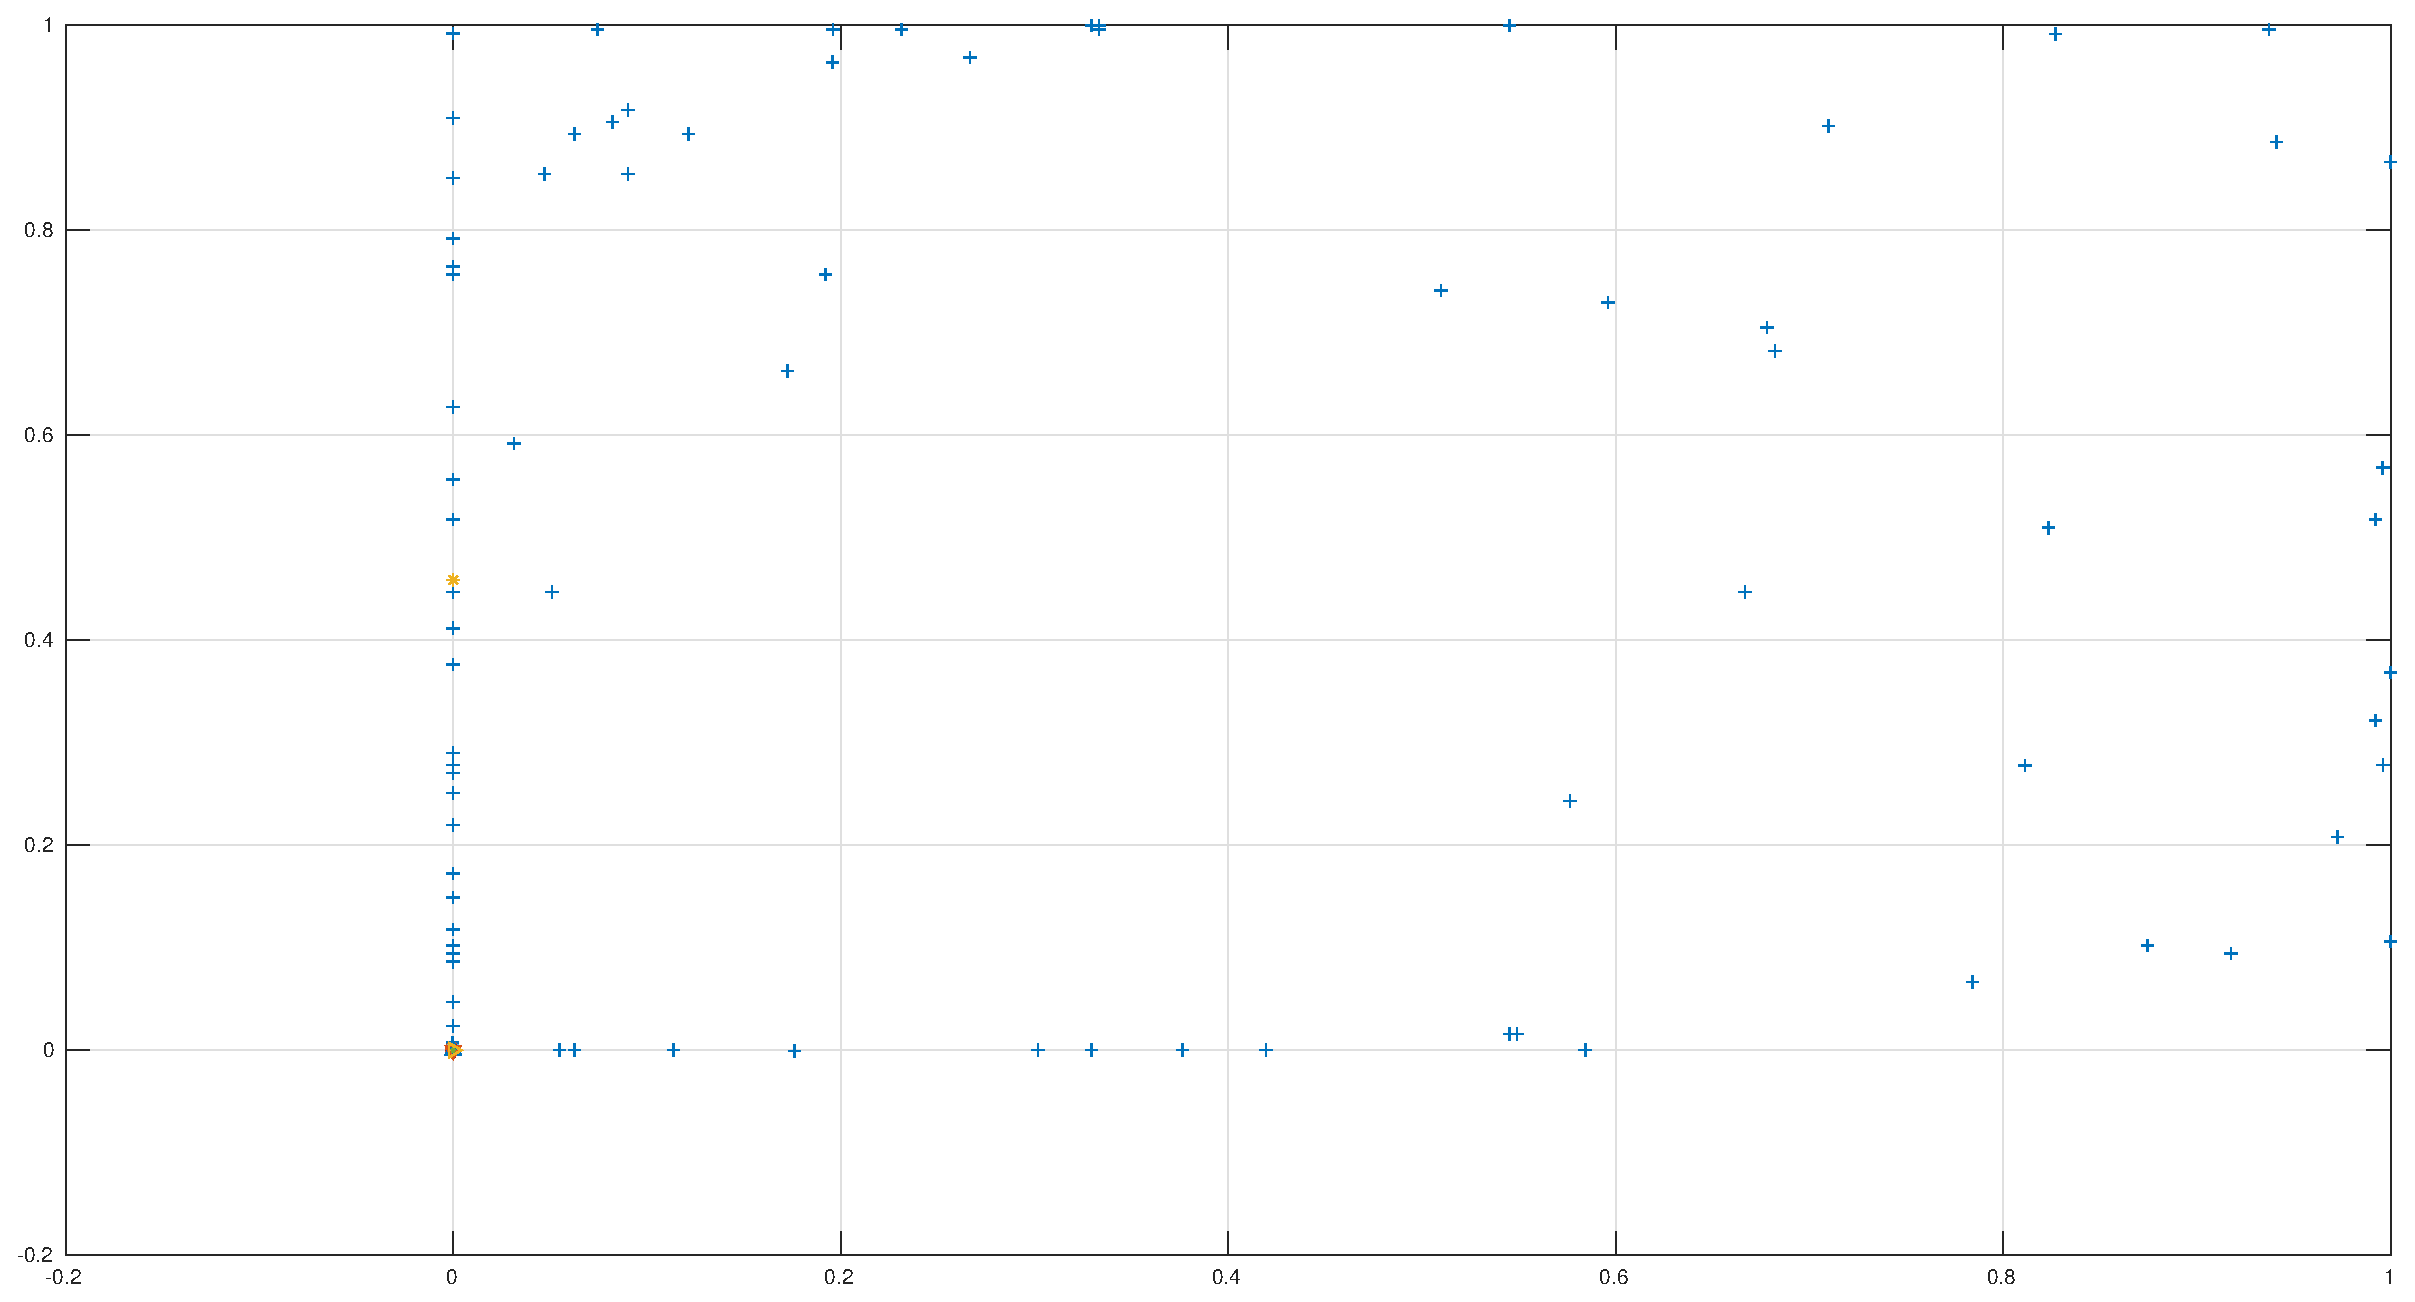
\includegraphics[width=0.5\textwidth]{plots/mnist_pca_plot.eps}}
  \caption{MNIST dataset after applying PCA}
\end{figure}
\begin{figure}[htbp]
  \centering
      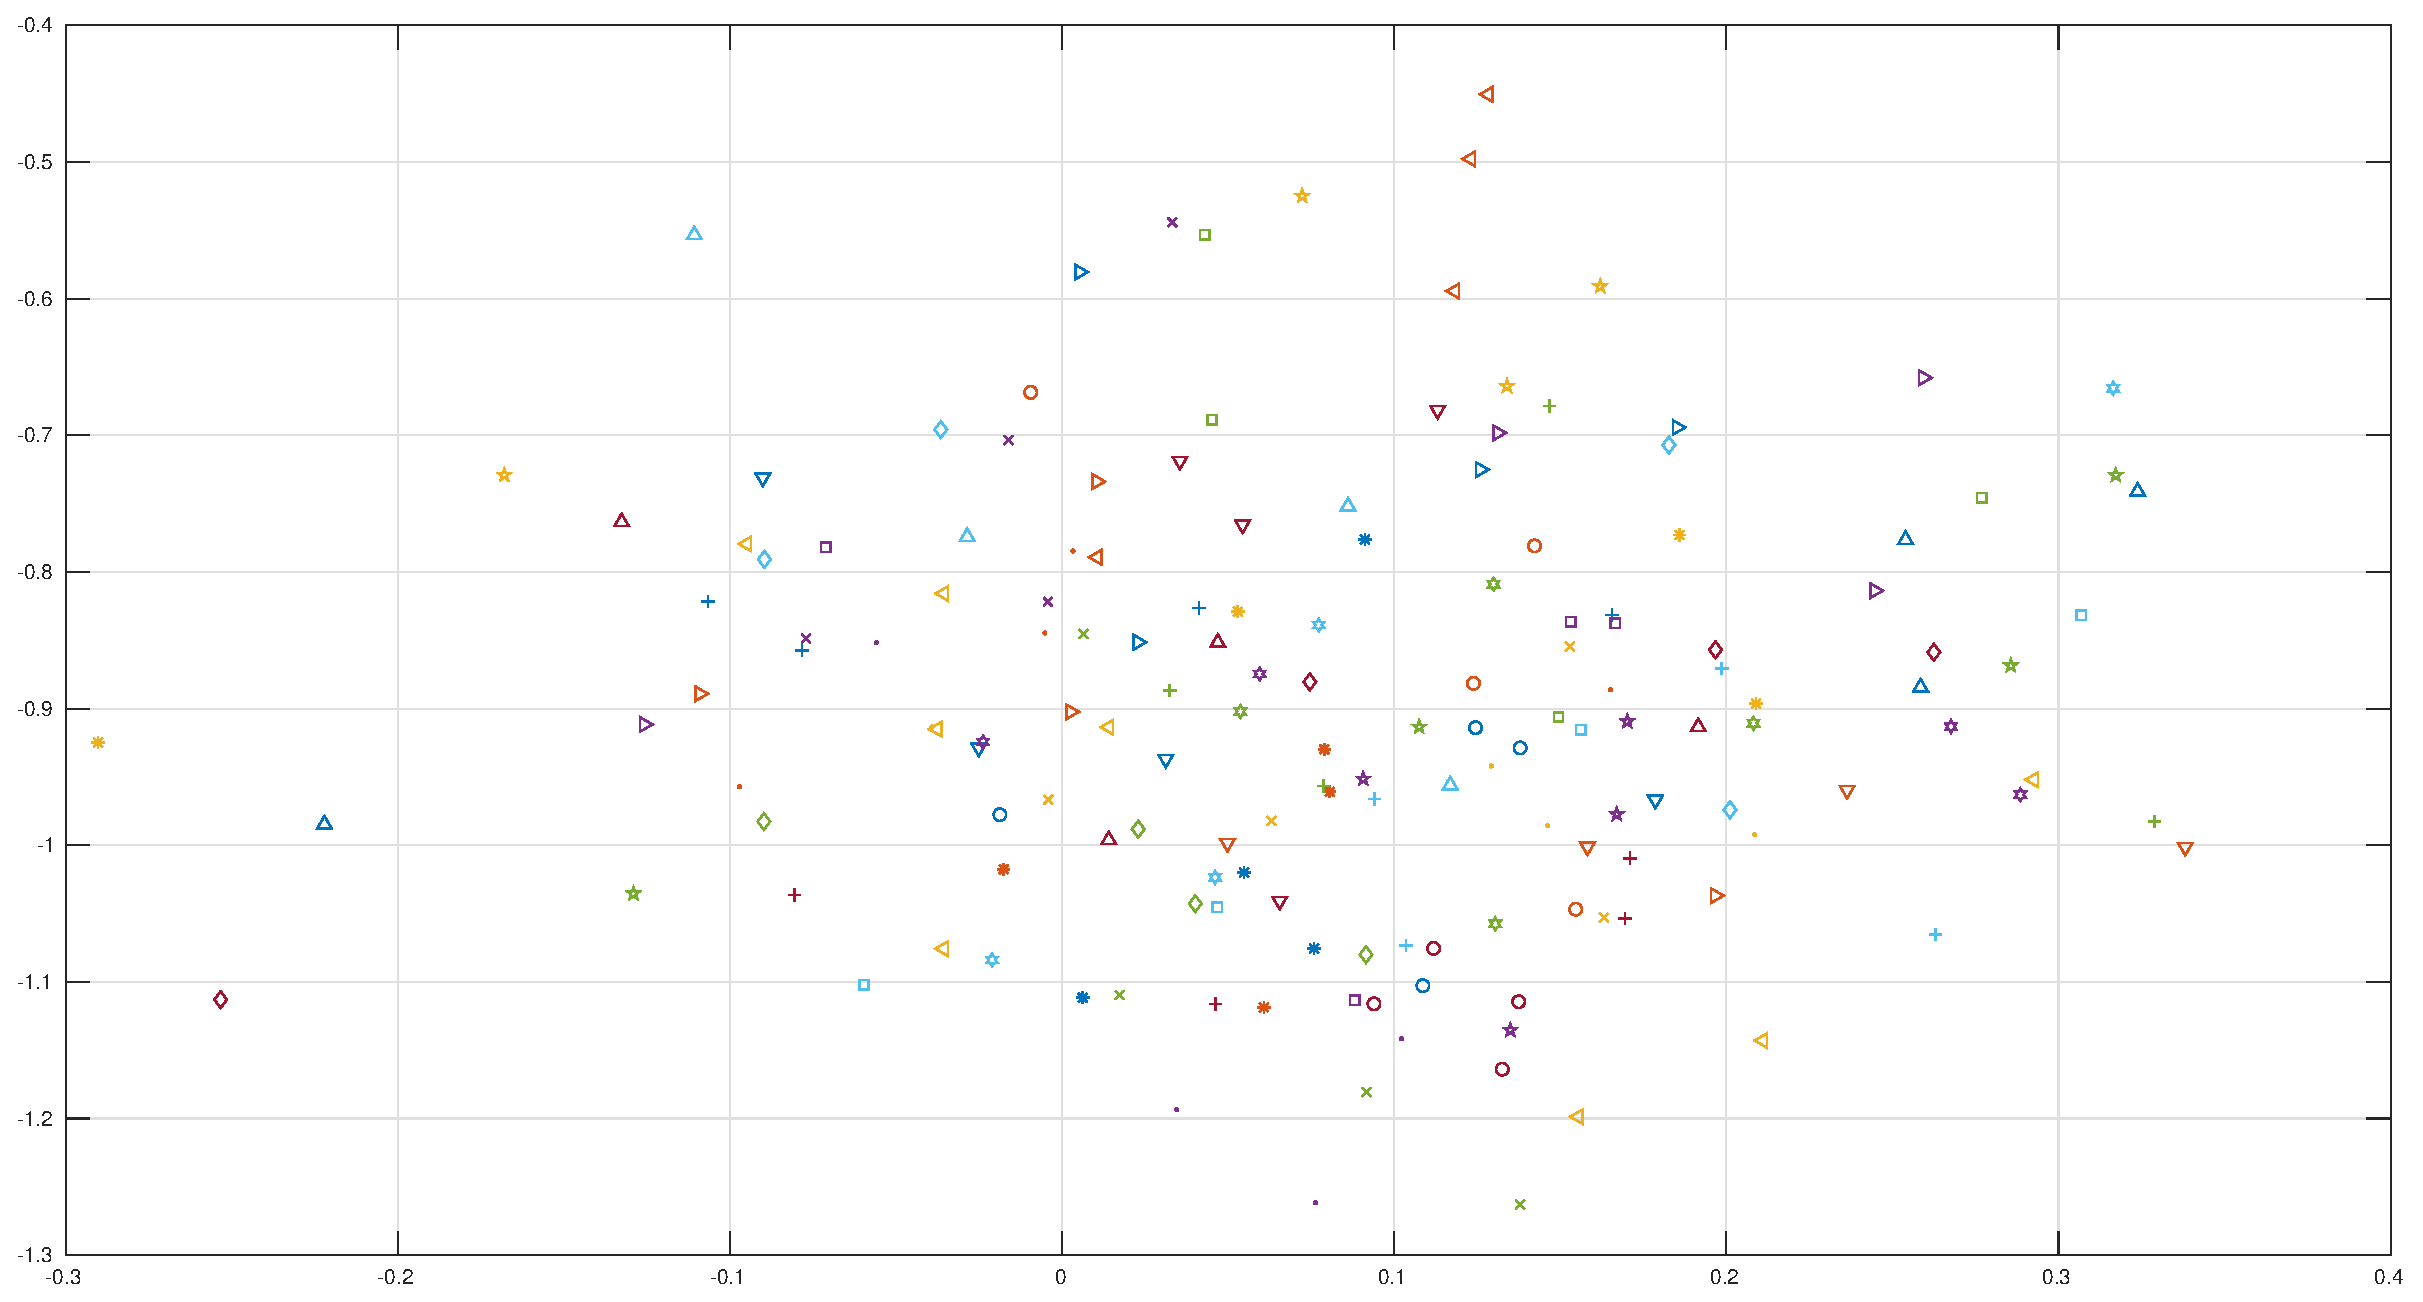
\includegraphics[width=0.5\textwidth]{plots/orl_pca_plot.eps}}
  \caption{ORL Data set after applying PCA}
\end{figure}


\section{Results}
As stated previously, each algorithm has been applied to the MNIST and ORL datasets. It is important to know that the MNIST dataset comes already split in training data (60000 samples) and test data (10000 samples), whereas the ORL dataset had to be manually and randomly split in 70\% training samples and 30\% test samples.

\tab The MNIST dataset is composed of 70000 pictures of handwritten digits in grayscale, from 0 to 9, and with an image resolution of 28x28.
\begin{figure}[htbp]
  \centering
      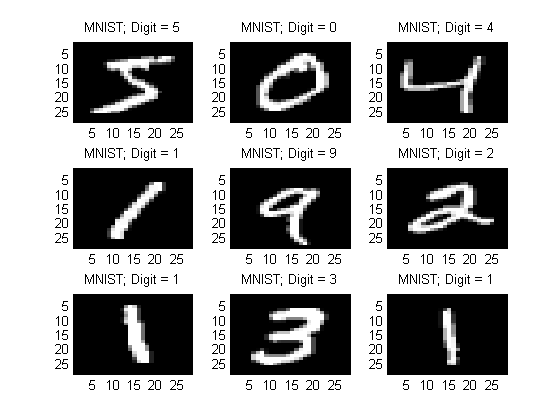
\includegraphics[width=0.5\textwidth]{mnist_example.png}}
  \caption{MNIST dataset sample}
\end{figure}

\tab The ORL dataset consists of 400 facial pictures, for it contains 10 pictures for each of the 40 persons, thus giving 40 classes.
\begin{figure}[htbp]
  \centering
      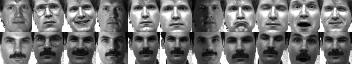
\includegraphics[width=0.4\textwidth]{orl.jpg}}
  \caption{ORL dataset sample}
\end{figure}

\tab Each algorithm has been compared by execution time, and success rate (or accuracy). It can be seen that changing the hyperparameters of one can drastically improve its success rate, as the Nearest Sub-class Centroid Classifier shows for instance, with the given hyperparameters \{2,3,5\} corresponding to the number of sub-classes. The learning rate for the backpropagation algorithm has been set to 0.1, after experimentation and fine-tuning.

\begin{figure}[htbp!]
  \centering
      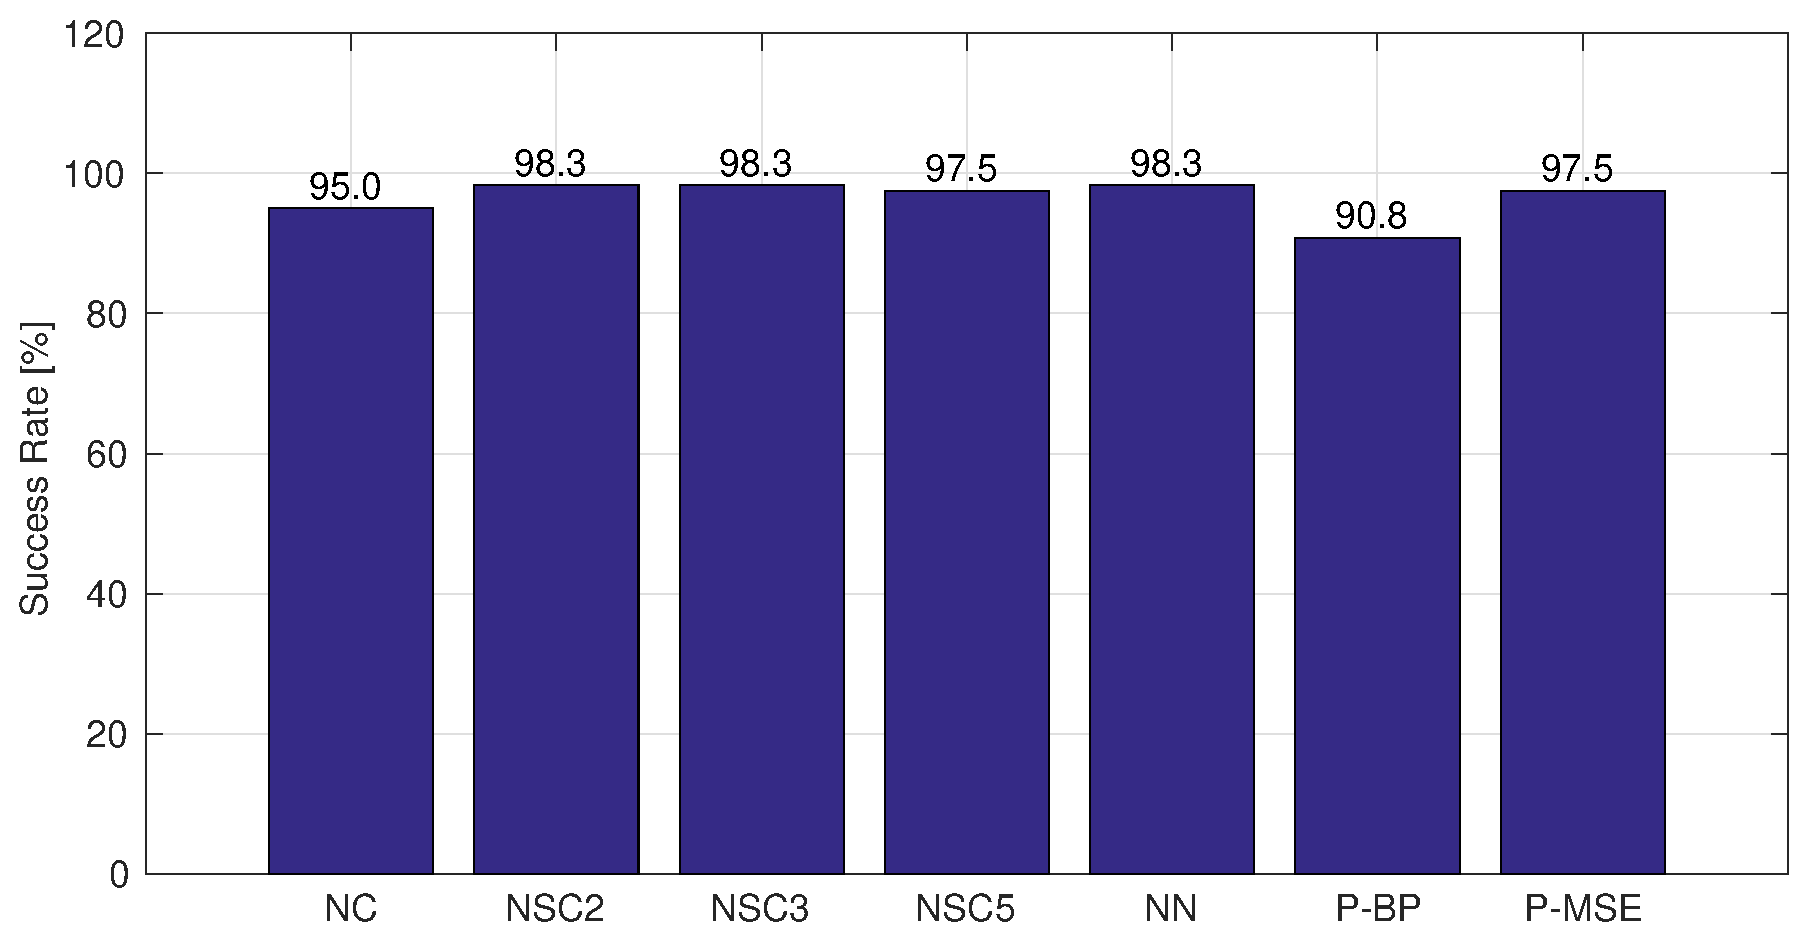
\includegraphics[width=0.5\textwidth]{plots/fig_ORL.eps}}
      \caption{ORL success rates}
\end{figure}

\\
\begin{figure}[htbp!]
  \centering
      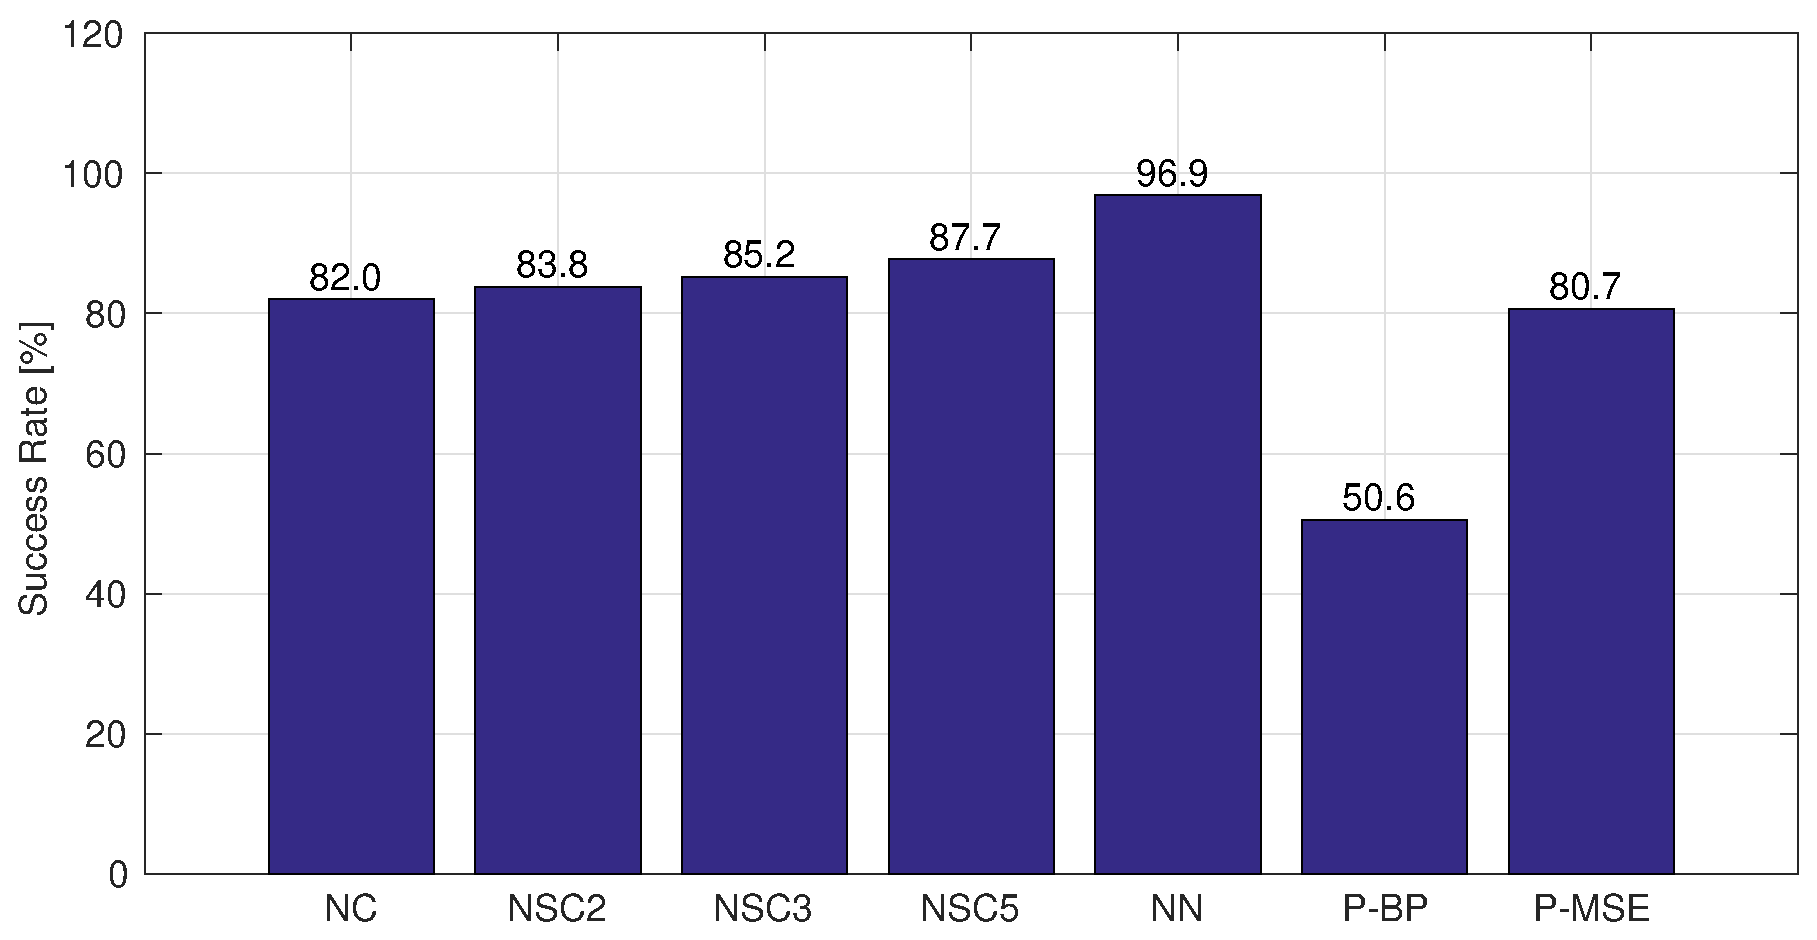
\includegraphics[width=0.5\textwidth]{plots/fig_MNIST.eps}}
      \caption{MNIST success rates}
\end{figure}


\tab The bar diagrams shown in figure 5 and 6 clearly demonstrate that most of the algorithms are more efficient and give slightly better results on the ORL dataset. It is also clear that the distance-based algorithms perform better than the perceptrons, and it is especially true for the Nearest Neighbour classifier, even though it is the slowest algorithm as shown in the following bar diagrams.


\tab As it can be seen on figure 7 and 8 of the conclusion section, the execution time of the Nearest Neighbour is the highest, as stated above, while the other distance-based classifiers globally remain the fastest to compute. In general, each algorithm is slightly slower to execute on the MNIST dataset, compared to the ORL dataset, and this is due to the fact that it is substantially larger than the latter. 

\tab The follong figures show the tremendous accuracy and processing time reduction after applying PCA to the datasets, thus reducing their dimensions to only 2. It goes without saying that applying PCA only to reduce the data's dimensions to 2D doesn't serve any interest other than constating the huge loss of accuracy. However, as the reduction of dimensions greatly reduces the execution time, it can be interesting to experiment with the amount of dimensions that the data can be reduced to, in order to obtain acceptable success rates while profiting from the great time gain.

% needed in second column of first page if using \IEEEpubid
%\IEEEpubidadjcol

% An example of a floating figure using the graphicx package.
% Note that \label must occur AFTER (or within) \caption.
% For figures, \caption should occur after the \includegraphics.
% Note that IEEEtran v1.7 and later has special internal code that
% is designed to preserve the operation of \label within \caption
% even when the captionsoff option is in effect. However, because
% of issues like this, it may be the safest practice to put all your
% \label just after \caption rather than within \caption{}.
%
% Reminder: the "draftcls" or "draftclsnofoot", not "draft", class
% option should be used if it is desired that the figures are to be
% displayed while in draft mode.
%
%\begin{figure}[!t]
%\centering
%\includegraphics[width=2.5in]{myfigure}
% where an .eps filename suffix will be assumed under latex, 
% and a .pdf suffix will be assumed for pdflatex; or what has been declared
% via \DeclareGraphicsExtensions.
%\caption{Simulation Results}
%\label{fig_sim}
%\end{figure}

% Note that IEEE typically puts floats only at the top, even when this
% results in a large percentage of a column being occupied by floats.


% An example of a double column floating figure using two subfigures.
% (The subfig.sty package must be loaded for this to work.)
% The subfigure \label commands are set within each subfloat command, the
% \label for the overall figure must come after \caption.
% \hfil must be used as a separator to get equal spacing.
% The subfigure.sty package works much the same way, except \subfigure is
% used instead of \subfloat.
%
%\begin{figure*}[!t]
%\centerline{\subfloat[Case I]\includegraphics[width=2.5in]{subfigcase1}%
%\label{fig_first_case}}
%\hfil
%\subfloat[Case II]{\includegraphics[width=2.5in]{subfigcase2}%
%\label{fig_second_case}}}
%\caption{Simulation results}
%\label{fig_sim}
%\end{figure*}
%
% Note that often IEEE papers with subfigures do not employ subfigure
% captions (using the optional argument to \subfloat), but instead will
% reference/describe all of them (a), (b), etc., within the main caption.


% An example of a floating table. Note that, for IEEE style tables, the 
% \caption command should come BEFORE the table. Table text will default to
% \footnotesize as IEEE normally uses this smaller font for tables.
% The \label must come after \caption as always.
%
%\begin{table}[!t]
%% increase table row spacing, adjust to taste
%\renewcommand{\arraystretch}{1.3}
% if using array.sty, it might be a good idea to tweak the value of
% \extrarowheight as needed to properly center the text within the cells
%\caption{An Example of a Table}
%\label{table_example}
%\centering
%% Some packages, such as MDW tools, offer better commands for making tables
%% than the plain LaTeX2e tabular which is used here.
%\begin{tabular}{|c||c|}
%\hline
%One & Two\\
%\hline
%Three & Four\\
%\hline
%\end{tabular}
%\end{table}


% Note that IEEE does not put floats in the very first column - or typically
% anywhere on the first page for that matter. Also, in-text middle ("here")
% positioning is not used. Most IEEE journals use top floats exclusively.
% Note that, LaTeX2e, unlike IEEE journals, places footnotes above bottom
% floats. This can be corrected via the \fnbelowfloat command of the
% stfloats package.



\section{Conclusion}
Finally, the algorithms' performances for both datasets can be visualized on the following graphs:
\begin{figure}[htbp]
  \centering
      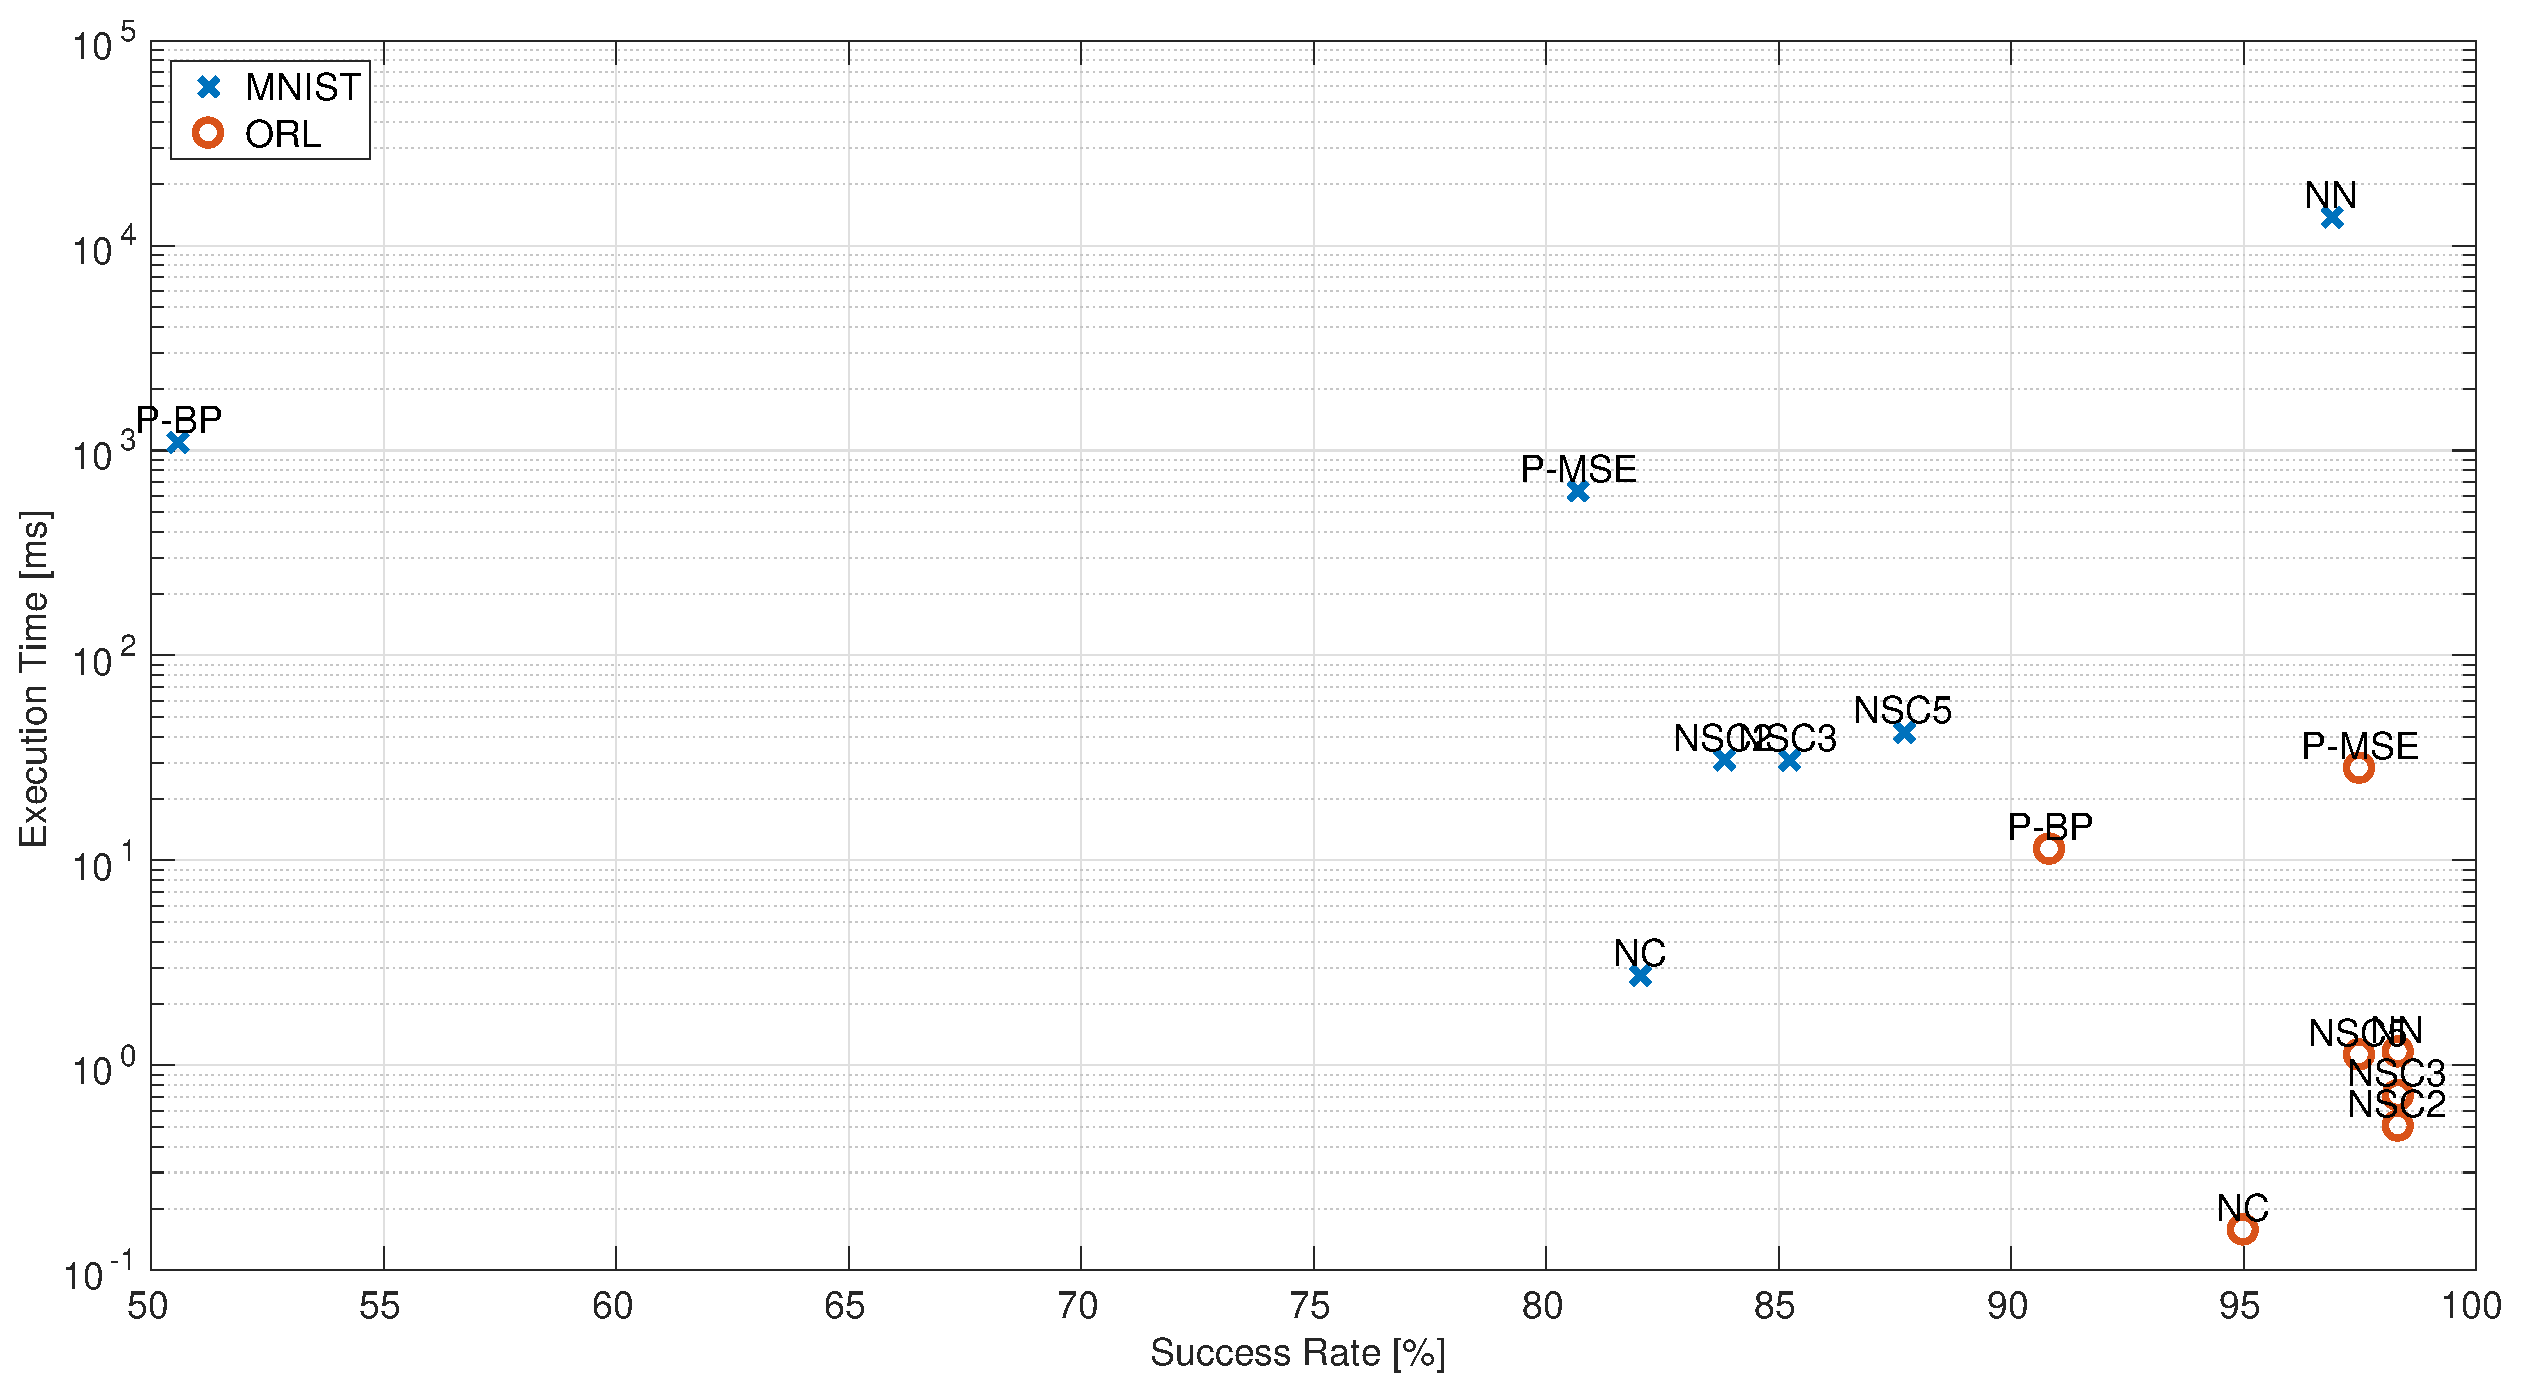
\includegraphics[width=0.5\textwidth]{plots/comparison_performance.eps}}
  \caption{Comparison of performance}
\end{figure}

\\
\begin{figure}[htbp]
  \centering
      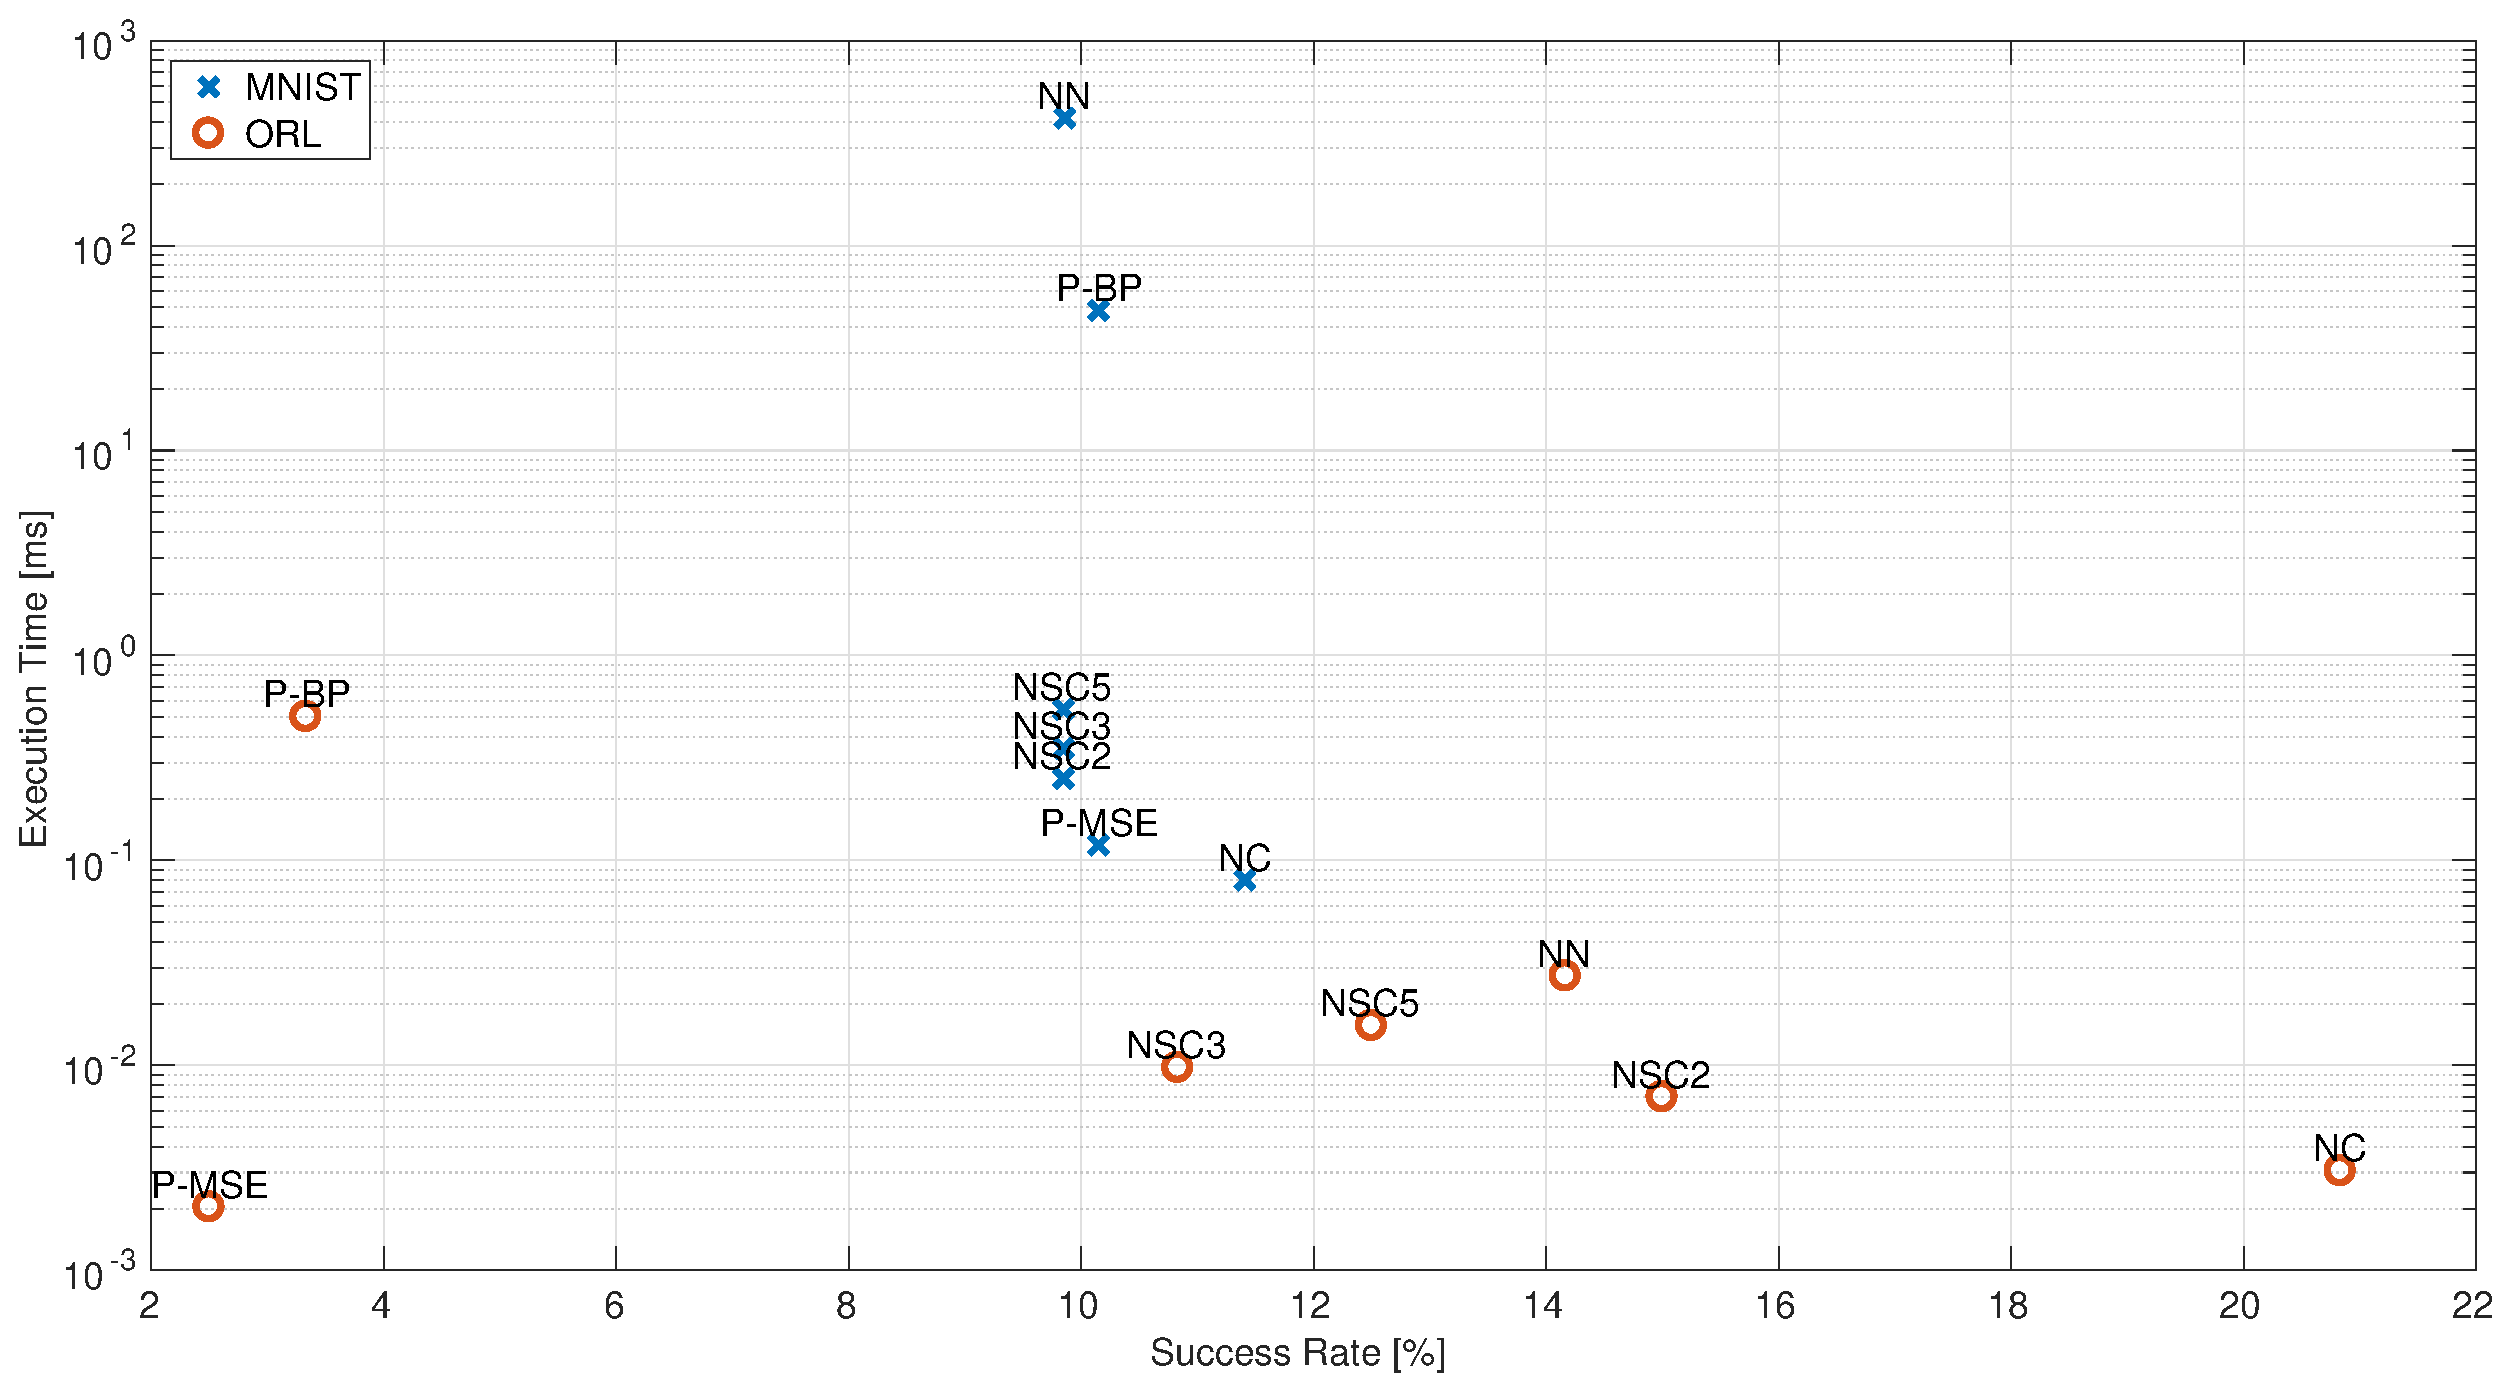
\includegraphics[width=0.5\textwidth]{plots/comparison_performance_pca.eps}}
  \caption{Comparison of performance after applying PCA}
\end{figure}
These figures represent the execution time and the success rates of each algorithm for each dataset (see legend). Of course, the higher accuracy the better, but a low execution time is very important as well, for real life applications.



\tab If more time was given for this project, it would have been a good thing to compare several iterations of the same algorithms for the ORL dataset for example, as the training samples and test samples are split randomly, thus resulting in very different results each time. Furthermore, this project was implemented in C++, and therefore took a lot more time than expected to be implemented, that is why the optimization has been set aside in order to obtain results quickly, and it would add a good value to work on the optimization, for example to make more use of threads (as it can be seen in the Nearest Neighbour Centroid) in every algorithm.





% if have a single appendix:
%\appendix[Proof of the Zonklar Equations]
% or
%\appendix  % for no appendix heading
% do not use \section anymore after \appendix, only \section*
% is possibly needed

% use appendices with more than one appendix
% then use \section to start each appendix
% you must declare a \section before using any
% \subsection or using \label (\appendices by itself
% starts a section numbered zero.)
%


\appendices
% use section* for acknowledgement

% Can use something like this to put references on a page
% by themselves when using endfloat and the captionsoff option.
\ifCLASSOPTIONcaptionsoff
  \newpage
\fi



% trigger a \newpage just before the given reference
% number - used to balance the columns on the last page
% adjust value as needed - may need to be readjusted if
% the document is modified later
%\IEEEtriggeratref{8}
% The "triggered" command can be changed if desired:
%\IEEEtriggercmd{\enlargethispage{-5in}}

% references section
% can use a bibliography generated by BibTeX as a .bbl file
% BibTeX documentation can be easily obtained at:
% http://www.ctan.org/tex-archive/biblio/bibtex/contrib/doc/
% The IEEEtran BibTeX style support page is at:
% http://www.michaelshell.org/tex/ieeetran/bibtex/
%\bibliographystyle{IEEEtran}
% argument is your BibTeX string definitions and bibliography database(s)
%\bibliography{IEEEabrv,../bib/paper}
%
% <OR> manually copy in the resultant .bbl file
% set second argument of \begin to the number of references
% (used to reserve space for the reference number labels box)

% biography section
% 
% If you have an EPS/PDF photo (graphicx package needed) extra braces are
% needed around the contents of the optional argument to biography to prevent
% the LaTeX parser from getting confused when it sees the complicated
% \includegraphics command within an optional argument. (You could create
% your own custom macro containing the \includegraphics command to make things
% simpler here.)
%\begin{biography}[{\includegraphics[width=1in,height=1.25in,clip,keepaspectratio]{mshell}}]{Michael Shell}
% or if you just want to reserve a space for a photo:

\end{IEEEbiography}

% You can push biographies down or up by placing
% a \vfill before or after them. The appropriate
% use of \vfill depends on what kind of text is
% on the last page and whether or not the columns
% are being equalized.

%\vfill

% Can be used to pull up biographies so that the bottom of the last one
% is flush with the other column.
%\enlargethispage{-5in}



% that's all folks
\end{document}


